\begin{frame}
	\frametitle{Hardware}
	\framesubtitle{The Evolution of a miniHPC}
	
	\begin{figure}
		\centering
		\begin{subfigure}[b]{0.24\textwidth}
			\centering
			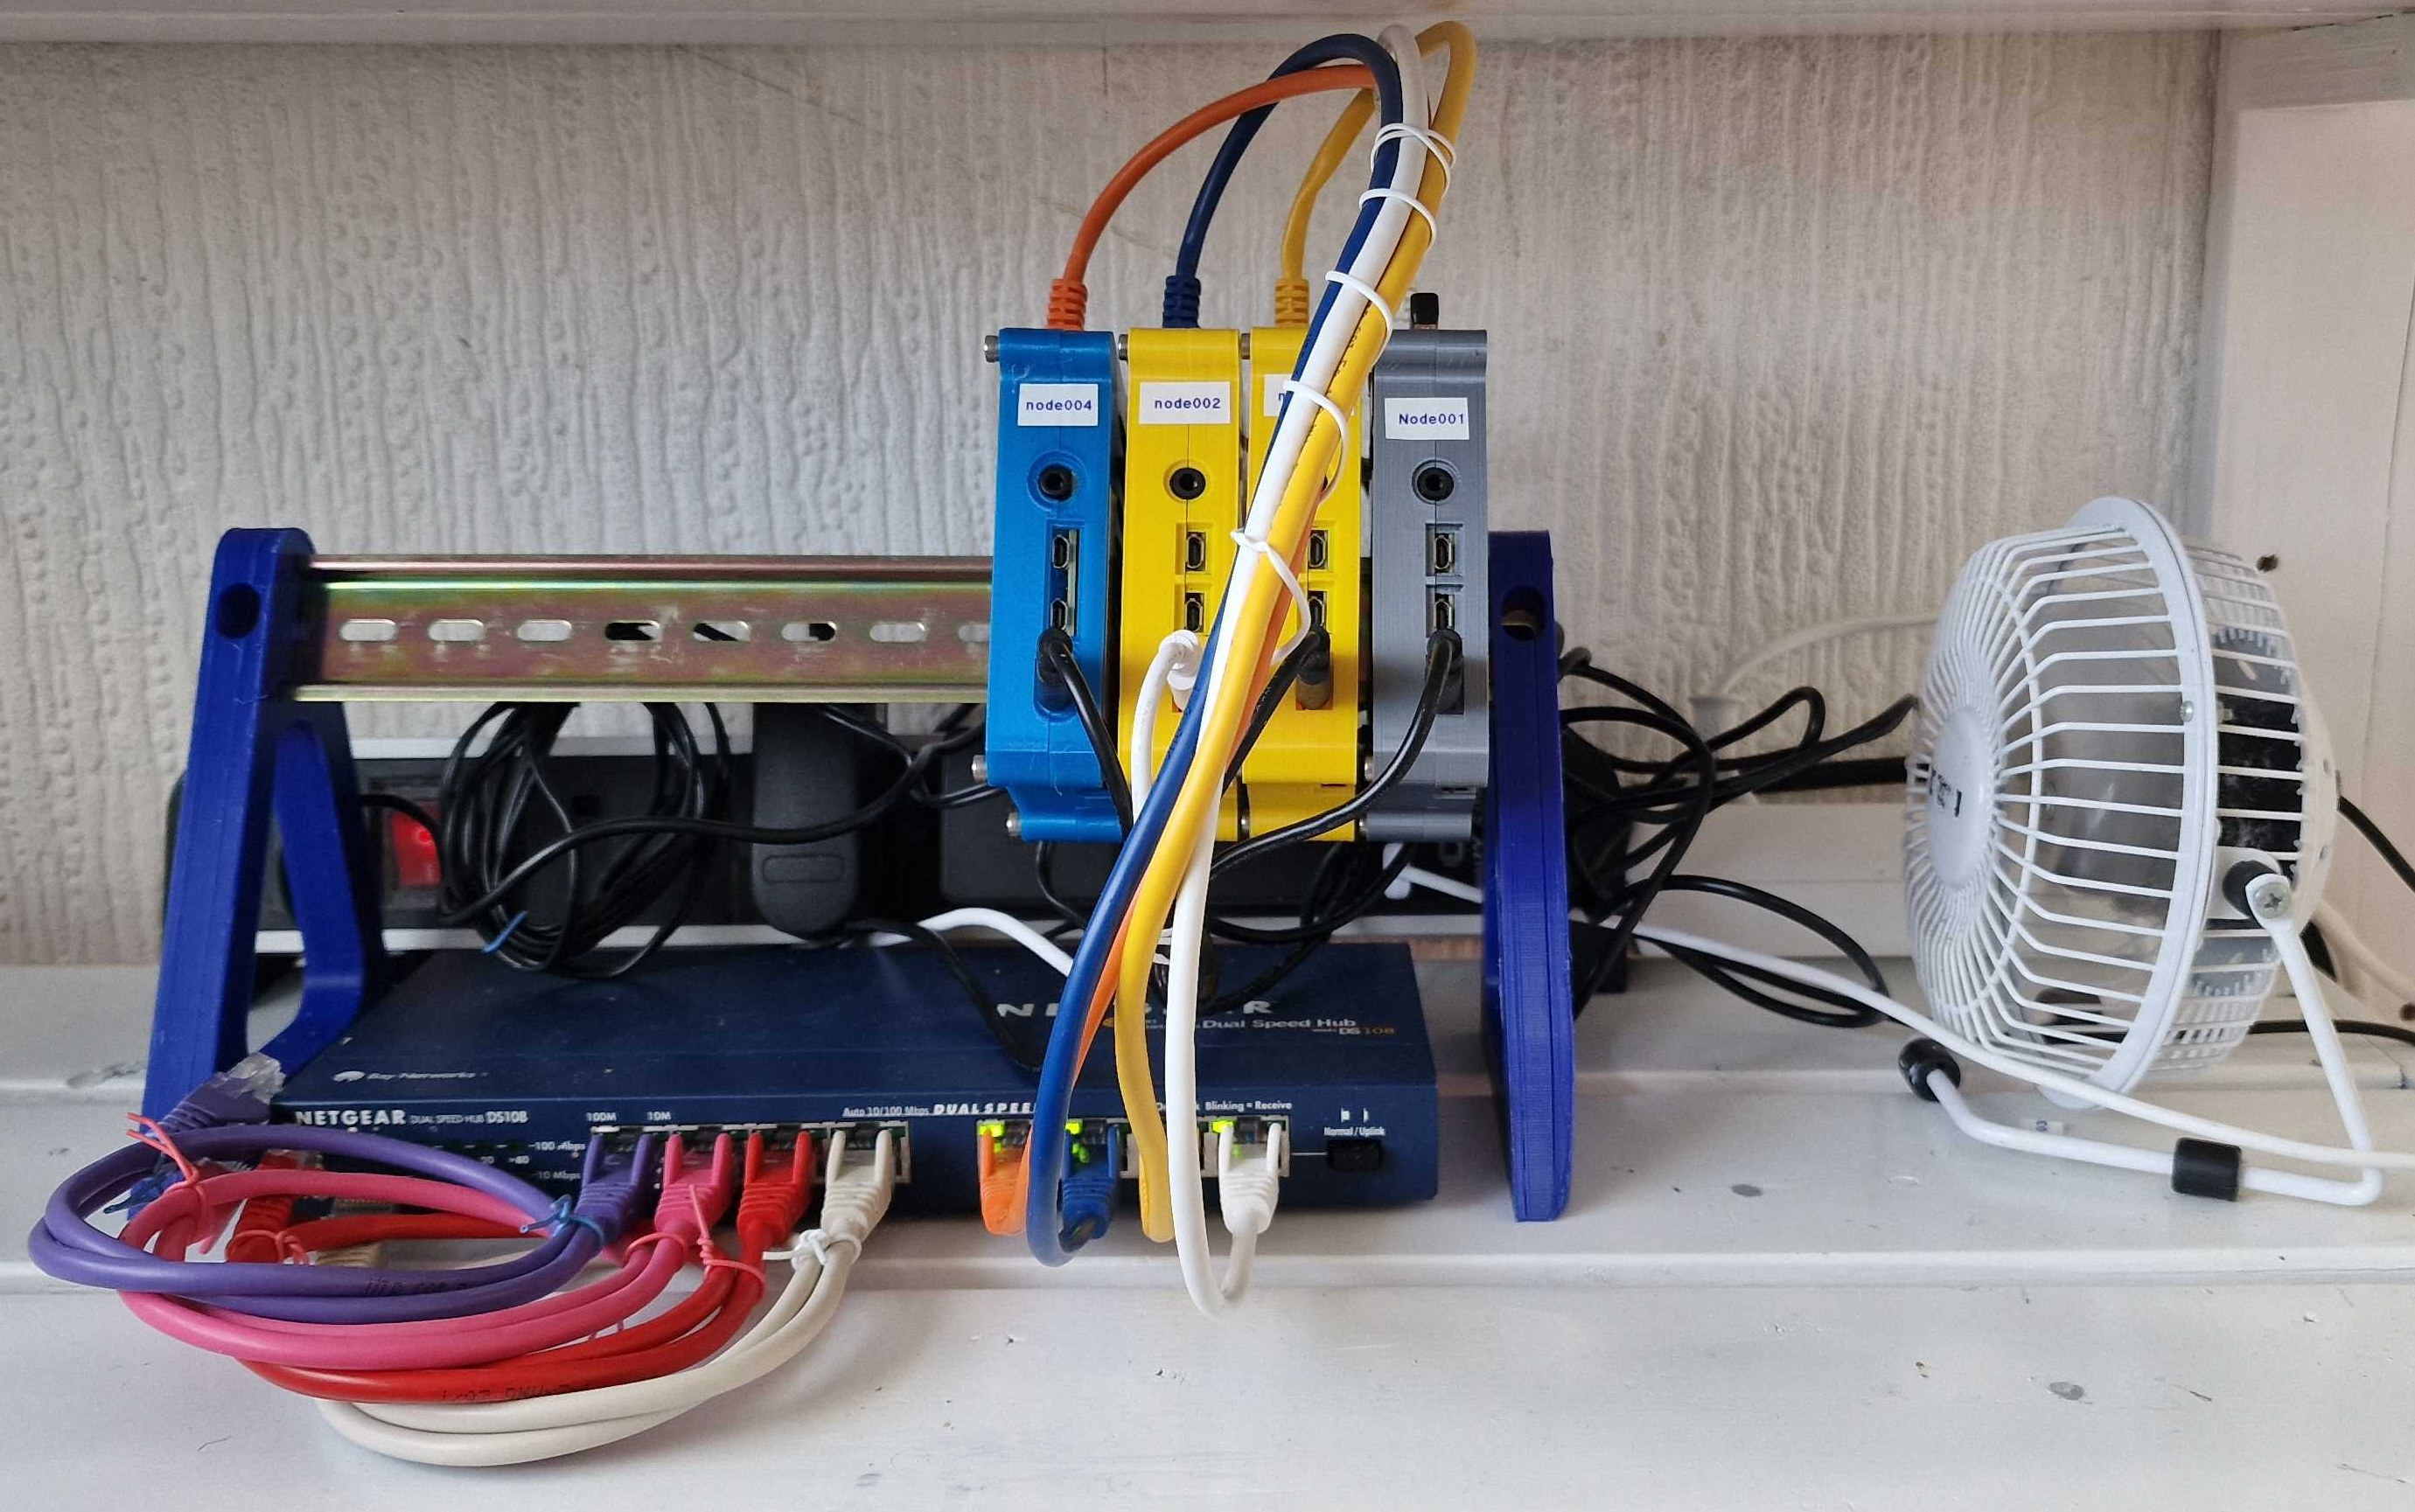
\includegraphics[width=\textwidth]{graphics/mini-HPC-proto1.png}
			\caption{Prototype 1}
			\label{fig:2.a}
		\end{subfigure}
		\hfill
		\begin{subfigure}[b]{0.24\textwidth}
			\centering
			\includegraphics[width=\textwidth]{graphics/mini-HPC-proto2.png}
			\caption{Prototype 2}
			\label{fig:2.b}
		\end{subfigure}
		\hfill
		\begin{subfigure}[b]{0.24\textwidth}
			\centering
			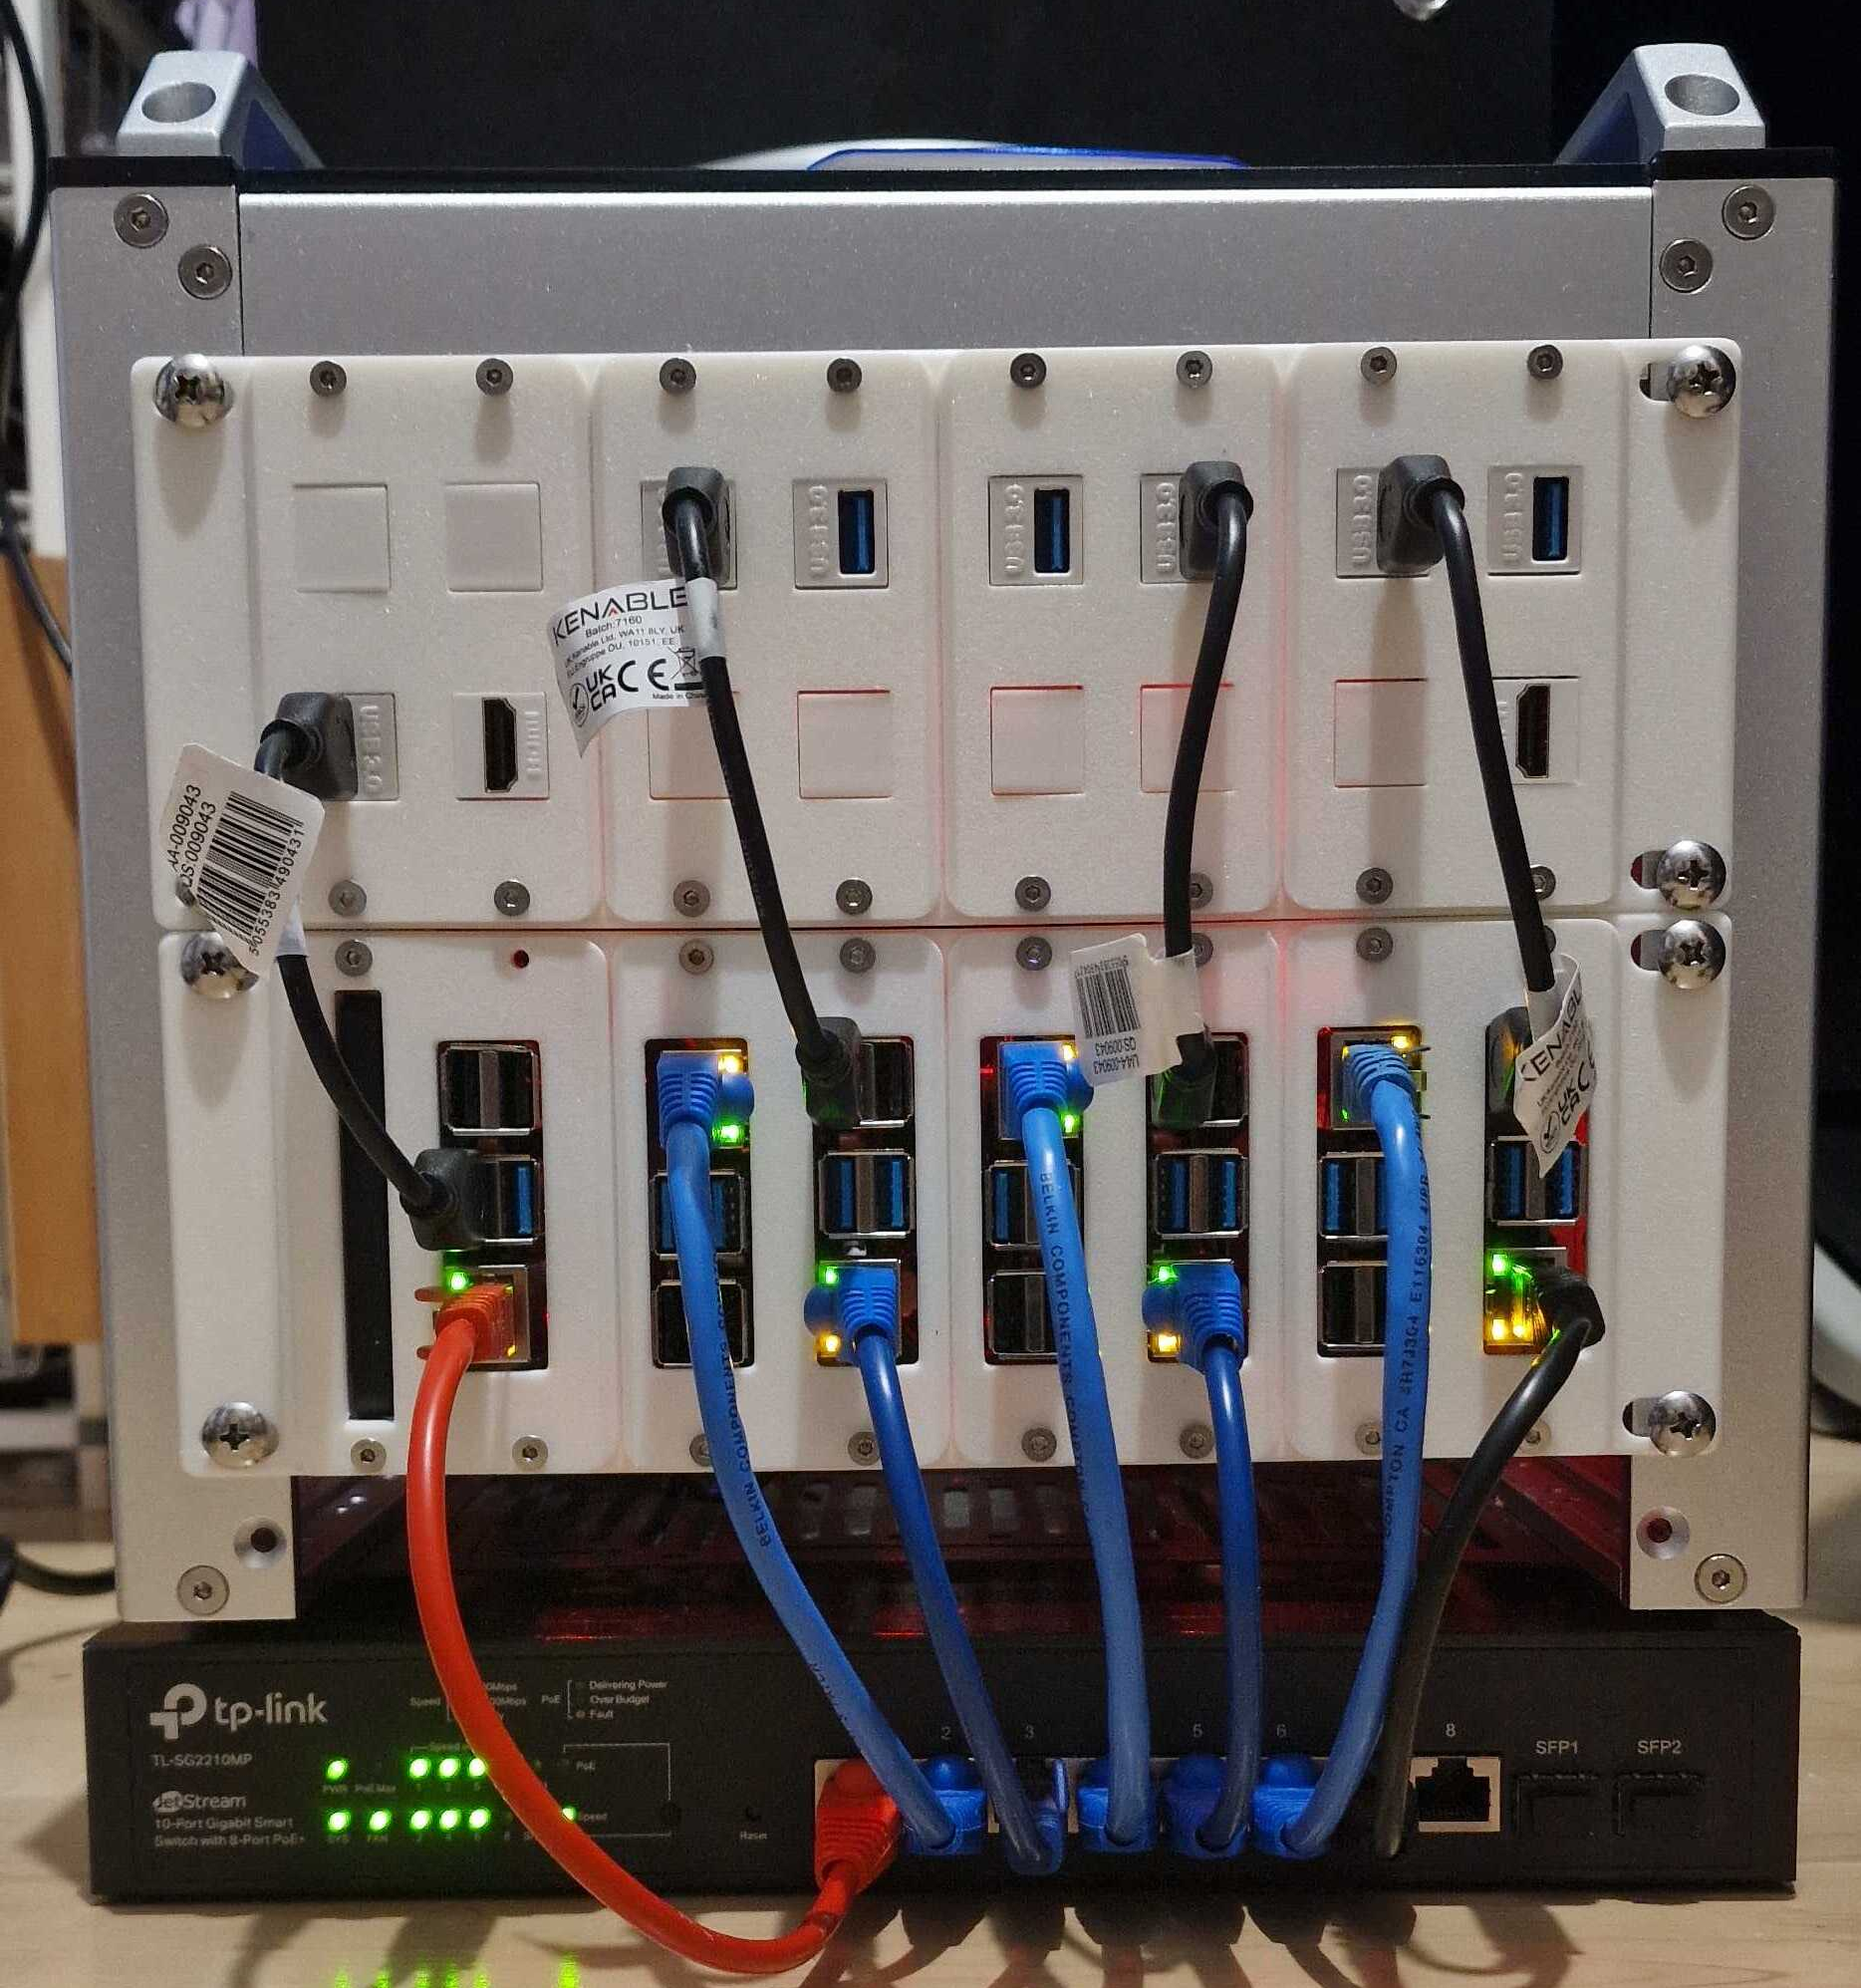
\includegraphics[width=\textwidth]{graphics/mini-HPC-proto3.png}
			\caption{Prototype 3 front}
			\label{fig:2.c}
		\end{subfigure}
		\hfill
		\begin{subfigure}[b]{0.24\textwidth}
			\centering
			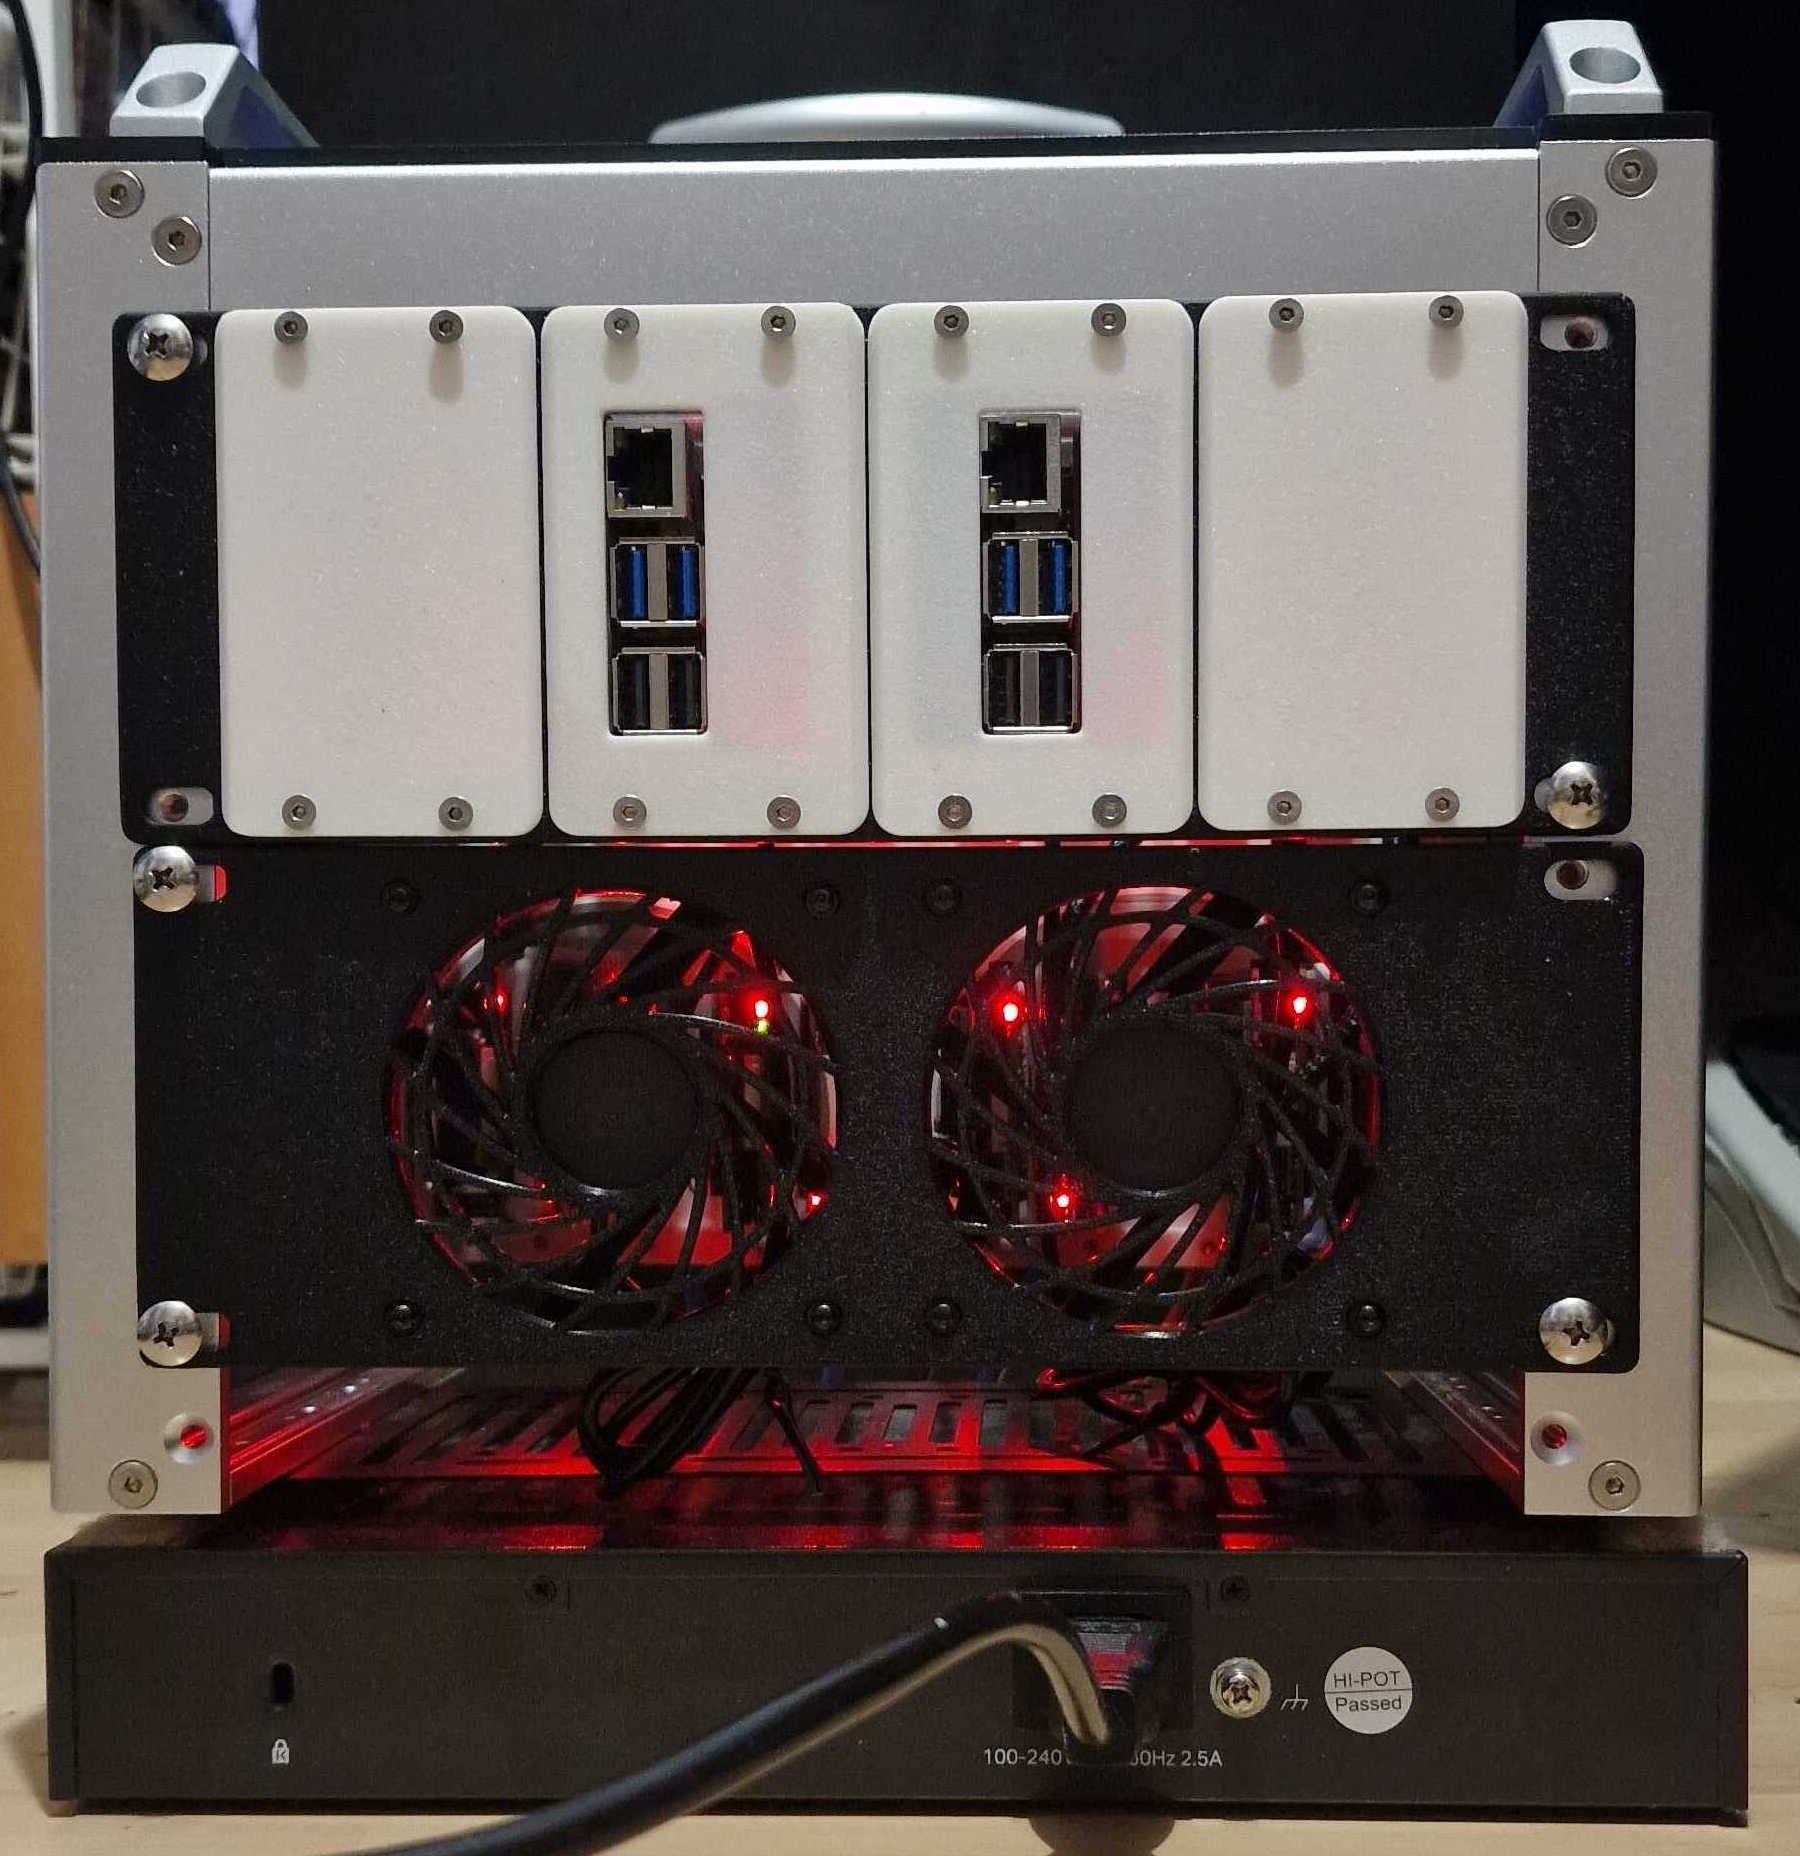
\includegraphics[width=\textwidth]{graphics/mini-HPC-proto3_back.png}
			\caption{Prototype 3 back}
			\label{fig:2.d}
		\end{subfigure}

		\label{fig:2}
	\end{figure}
	
\end{frame}
